\documentclass[12pt]{article}

\usepackage[a4paper,top=1in,bottom=1in,left=1in,right=1in]{geometry}

\usepackage[utf8]{inputenc}
\usepackage{float}
\usepackage{amsmath}
\usepackage{graphicx}
\usepackage{titlesec}
\usepackage{tcolorbox}
\usepackage{enumitem}
\usepackage{tikz}
\usetikzlibrary{patterns}
\usetikzlibrary{graphs}
\usetikzlibrary{graphdrawing}
\usegdlibrary{force}
\usepackage{amssymb}
\usepackage{hyperref}

\title{\bfseries Laborator Proiectare Logică 5}
\author{Sîrghe Matei}
\date{October 30, 2024}

\titleformat{\section}
  {\normalfont\Large\bfseries}{\thesection}{1em}{}
\begin{document}
\maketitle

\begin{center}
    \large{\textbf{Optimizarea funcțiilor logice}}
\end{center}
\begin{center}
    \large{\textbf{Optimizarea-reducerea numărului de operații}}
\end{center}

\renewcommand{\arraystretch}{1}

\begin{center}
    \textbf{Exerciții}
\end{center}

\begin{figure}[h!]
    \begin{minipage}{0.8\textwidth}
        \textbf{Exercițiul 1:\\}
        $y: 2^3 \rightarrow 2^1$;
        $y = \sum(1,2,3,5,6)=FCD_{y}$\\
        $y = \Pi(0,4,7)=FCC_{y} $\\
        $FCD_{y}=\bar{A}\bar{B}C+\bar{A}B\bar{C}+\bar{A}BC+A\bar{B}C+AB\bar{C}$\\
        21 operații logice $\uparrow$\\
        $FCC_{y}=(A+B+C)(\bar{A}+B+C)(\bar{A}+\bar{B}+\bar{C})$\\
        12 operații logice $\uparrow$\\
        \textbf{Rezolvare:}
        $FCD_{y}=\sum(2,3)=n(2,3)=A\bar{B}+AB$\\
        $ FCC_{y}=\Pi(0,1)=m(0,1)=(A+B)(A+\bar{B}) $\\
        $ y= A\bar{B}+AB=A(\bar{B}+B)=A\times1=A$\\
        $y=(A+B)(A+\bar{B})=A^2+A\bar{B}+BA+B\bar{B}$\\
        $ =A+A\bar{B}+AB+0=A(1+B+\bar{B})=A$\\
    \end{minipage}
    \hfill
    \begin{minipage}{0.18\textwidth}
        \begin{tabular}{|c|c|c|c|}
            \hline
            A & B & C & y \\ \hline
            0 & 0 & 0 & 0 \\ \hline
            0 & 0 & 1 & 1 \\ \hline
            0 & 1 & 0 & 1 \\ \hline
            0 & 1 & 1 & 1 \\ \hline
            1 & 0 & 0 & 0 \\ \hline
            1 & 0 & 1 & 1 \\ \hline
            1 & 1 & 0 & 1 \\ \hline
            1 & 1 & 1 & 0 \\ \hline
        \end{tabular}
    \end{minipage}
\end{figure}


\begin{figure}[h!]
    \begin{minipage}{0.5\textwidth}
        \begin{tikzpicture}
            \draw (0.75,1) circle [radius=1cm];
            \draw (-0.75,1) circle [radius=1cm];
            \draw (0,-0.25) circle [radius=1cm];
            \fill[pattern=north east lines] (0.75,1) circle [radius=1cm];
            \fill[pattern=north east lines] (0,-0.25) circle [radius=1cm];
        
            \node at (0.75,1) {B};
            \node at (-0.75,1) {A};
            \node at (0,-0.25) {C};
        \end{tikzpicture}
    \end{minipage}
    \hfill
    \begin{minipage}{0.5\textwidth}
        \begin{tikzpicture}
            % Draw the table grid
            \draw (0,0) grid (4,-2);
            
            % Label columns
            \node at (0.5, 0.5) {$\bar{A}$};
            \node at (1.5, 0.5) {$\bar{A}$};
            \node at (2.5, 0.5) {$A$};
            \node at (3.5, 0.5) {$A$};
        
            \draw[thick] (2, -0.5) ellipse (1cm and 0.5cm);
            \draw[thick] (1.5, -1) ellipse (0.5cm and 1cm);

            \draw[thick] (4,-2) arc[start angle=270, end angle=90, x radius=1cm, y radius=0.5cm];
            \draw[thick] (0,-1) arc[start angle=90, end angle=-90, x radius=1cm, y radius=0.5cm];

            \node at (0.5, -0.5) {0};
            \node at (1.5, -0.5) {1};
            \node at (2.5, -0.5) {1};
            \node at (3.5, -0.5) {0};
            %
            \node at (0.5, -1.5) {1};
            \node at (1.5, -1.5) {1};
            \node at (2.5, -1.5) {0};
            \node at (3.5, -1.5) {1};

            % Label rows
            \node at (-0.5, -0.5) {$\bar{C}$};
            \node at (-0.5, -1.5) {C};

             % Label columns
             \node at (0.5, -2.5) {$\bar{B}$};
             \node at (1.5, -2.5) {$B$};
             \node at (2.5, -2.5) {$B$};
             \node at (3.5, -2.5) {$\bar{B}$};
        \end{tikzpicture}
    \end{minipage}
\end{figure}

$\bar{A}(\bar{B}C+B\bar{C})+A(\bar{B}C+B\bar{C})+\bar{A}(BC)$\\
$=(\bar{A}+A)(\bar{B}C+B\bar{C})+\bar{A}BC$\\
$=\bar{B}C+B\bar{C}+\bar{A}BC$\\
$=B\bigoplus C +\bar{A}BC$\\

\begin{figure}[H]
    \begin{minipage}{0.4\textwidth}
        \textbf{Exercițiul 2:\\}
        Faceți schema pentru funția:\\
        $y=B\bar{C}+\bar{A}B+C\bar{B}$\\
    \end{minipage}
    \hfill
    \begin{minipage}{0.5\textwidth}
        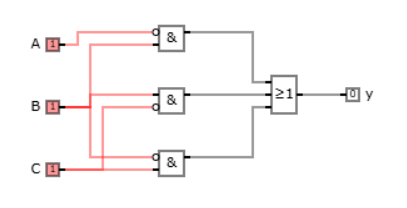
\includegraphics[scale=0.8]{schema1.png}
    \end{minipage}
\end{figure}

\begin{figure}[H]
    \begin{minipage}{0.7\textwidth}
        \textbf{Exercițiul 3:\\}
        Simplificați funcția dată prin tabela de adevăr:\\
        \textbf{Rezolvare:\\}
        $y=\sum(0,2,3,4,5,6,8,9,10,12)$\\
        $ = \bar{A}\bar{B}\bar{C}\bar{D}+\bar{A}\bar{B}C\bar{D}+\bar{A}\bar{B}CD+\bar{A}B\bar{C}\bar{D}+$\\
        $ + \bar{A}B\bar{C}D+A\bar{B}\bar{C}\bar{D}+A\bar{B}\bar{C}\bar{D}+A\bar{B}\bar{C}D+A\bar{B}C\bar{D}+AB\bar{C}\bar{D} $\\
        $y=\Pi(1,7,11,13,14,15)$\\
        $ =(A+B+C+\bar{D})(A+\bar{B}+\bar{C}+\bar{D})(\bar{A}+B+\bar{C}+\bar{D})$\\
        $ (\bar{A}+\bar{B}+C+\bar{D})(\bar{A}+\bar{B}+\bar{C}+D)(\bar{A}+\bar{B}+\bar{C}+\bar{D})$\\
    \end{minipage}
    \hfill
    \begin{minipage}{0.18\textwidth}
        \begin{tabular}{|c|c|c|c|c|}
            \hline
            A & B & C & D & y \\ \hline
            0 & 0 & 0 & 0 & 1 \\ \hline
            0 & 0 & 0 & 1 & 0 \\ \hline
            0 & 0 & 1 & 0 & 1 \\ \hline
            0 & 0 & 1 & 1 & 1 \\ \hline
            0 & 1 & 0 & 0 & 1 \\ \hline
            0 & 1 & 0 & 1 & 1 \\ \hline
            0 & 1 & 1 & 0 & 1 \\ \hline
            0 & 1 & 1 & 1 & 0 \\ \hline
            1 & 0 & 0 & 0 & 1 \\ \hline
            1 & 0 & 0 & 1 & 1 \\ \hline
            1 & 0 & 1 & 0 & 1 \\ \hline
            1 & 0 & 1 & 1 & 0 \\ \hline
            1 & 1 & 0 & 0 & 1 \\ \hline
            1 & 1 & 0 & 1 & 0 \\ \hline
            1 & 1 & 1 & 0 & 0 \\ \hline
            1 & 1 & 1 & 1 & 0 \\ \hline
        \end{tabular}
    \end{minipage}
\end{figure}

\begin{figure}[H]
    \begin{minipage}{0.6\textwidth}
        \begin{tikzpicture}
            \draw (0,0) grid (4,-4);
        
            \draw[thick] (2, -0.5) ellipse (2cm and 0.5cm);
            \draw[thick] (1.5, -1.5) ellipse (0.5cm and 0.5cm);
            \draw[thick] (3.5, -1.5) ellipse (0.5cm and 0.5cm);
            \draw[thick] (1, -3.5) ellipse (1cm and 0.5cm);
            \draw[thick] (0.5, -3) ellipse (0.5cm and 1cm);
            \draw[thick] (3.5, -3.5) ellipse (0.5cm and 0.5cm);
        
            \node at (0.5, -0.5) {1};
            \node at (1.5, -0.5) {1};
            \node at (2.5, -0.5) {1};
            \node at (3.5, -0.5) {1};
            %
            \node at (0.5, -1.5) {0};
            \node at (1.5, -1.5) {1};
            \node at (2.5, -1.5) {0};
            \node at (3.5, -1.5) {1};
            %
            \node at (0.5, -2.5) {1};
            \node at (1.5, -2.5) {0};
            \node at (2.5, -2.5) {0};
            \node at (3.5, -2.5) {0};
            %
            \node at (0.5, -3.5) {1};
            \node at (1.5, -3.5) {1};
            \node at (2.5, -3.5) {0};
            \node at (3.5, -3.5) {1};
        
            \node at (0.5, 0.5) {$\bar{A}$};
            \node at (1.5, 0.5) {$\bar{A}$};
            \node at (2.5, 0.5) {$A$};
            \node at (3.5, 0.5) {$A$};
        
            \node at (-0.5, -0.5) {$\bar{C}$};
            \node at (-0.5, -1.5) {$\bar{C}$};
            \node at (-0.5, -2.5) {C};
            \node at (-0.5, -3.5) {C};
        
            \node at (4.5, -0.5) {$\bar{D}$};
            \node at (4.5, -1.5) {D};
            \node at (4.5, -2.5) {D};
            \node at (4.5, -3.5) {$\bar{D}$};
        
             \node at (0.5, -4.5) {$\bar{B}$};
             \node at (1.5, -4.5) {$B$};
             \node at (2.5, -4.5) {$B$};
             \node at (3.5, -4.5) {$\bar{B}$};
        \end{tikzpicture}
    \end{minipage}
    \hfill
    \begin{minipage}{0.4\textwidth}
        $y=\bar{C}\bar{D}+\bar{A}B\bar{C}D+A\bar{B}\bar{C}D+\bar{A}\bar{B}C+\bar{A}C\bar{D}+A\bar{B}C\bar{D}$\\
    \end{minipage}
\end{figure}

\end{document}